\documentclass[a4paper,norsk,12pt]{article}

\usepackage[norsk]{babel}
\usepackage{enumitem}
\usepackage{color}
\usepackage{amsmath}
\usepackage{wrapfig}
\usepackage{graphicx}
\usepackage[utf8]{inputenc}
\usepackage{multirow,tabularx}
\usepackage{setspace}
\usepackage{hyperref}
\onehalfspacing
\newcolumntype{Y}{>{\centering\arraybackslash}X}
\renewcommand{\arraystretch}{2}

\pagestyle{empty}

\begin{document}
\section{Bakgrunn og teorigrunnlag}
Læringsforskning viser at undervisning basert på kun forelesninger, regne\-øvinger og laboratorie-øvinger---noe som ofte er tilfellet for introduksjonskurs i blant annet fysikk på universitet/høyskole-nivå---i liten grad øker de studenters forståelse av fundamentale konsepter~\cite{doi:10.1119/1.14030, doi:10.1119/1.18809, doi:10.1119/1.18863}. Studiene har ikke bare undersøkt læringsutbyttet av de tradisjonelle undervisningsformene, men også foretatt en kvantitativ sammenligning med undervisning basert på mer student\-aktive læringsformer. Von Korff og medarbeider~\cite{doi:10.1119/1.4964354} har publisert en metastudie som oppsummerer resultatene fra læringsanalyse i grunnleggende fysikk som omfatter 45\,000 studenter i perioden 1995 til 2014. Studentene i de 72 undersøkelsene som er inkludert i metastudien tok alle introduksjonskurs i klassisk mekanikk ved et college eller universitet i USA eller Canada. Hovedkonklusjonen fra denne metastudien er at studentaktive læringsformer gir signifikant høyere læringsutbytte en tradisjonelle forelesninger. Videre fant de at det var relativt stor variasjon i læringsutbyttet i ulike klasser---både der tradisjonelle forelesninger og der studentaktive læringsformer ble benyttet. Metastudien finner ikke evidens for at denne variasjonen i læringsutbytte kan forklares ved klassestørrelse, institusjonstype (f.eks.~eliteuniversitet sammenlignet med mindre colleger), SAT-score\footnote{Standardisert testing som brukes ved opptak til amerikanske universiteter og colleger.}, eller ferdighetsnivå i fysikk ved starten av studien målt gjennom resultatet på en test før undervisningsperioden. Merk at denne sammenligninen bruker gjennomsnittsverdien for hele klassen. Det er derfor mulig at enkelte av variablene som ble funnet å ikke ha signifikant effekt likevel kan være av betydning på enkeltstudent-nivå.

I en studie gjort ved Cal Poly i California, USA, ble læringsutbyttet av tradisjonelle forelseninger sammenlignet med det fra studentaktiv læring\footnote{Studentaktiv læring var her realisert gjennom "studio classroom" der studentene ikke møter forelesninger i det hele tatt, men bruker tiden på å jobbe sammen med eksperimenter og å løse øvingsoppgaver.} med et studiedesign som tillot dem å ta bort hvem som foreleste for de ulike klassen som faktor \cite{FiveEasyLessons}. Dette oppnådde de ved at alle tre underviserne som deltok i studien både hadde ansvaret for en klasse med forelesningsbasert undervisning og en klasse med studentaktiv undervisning. Underviserne i studien var valgt ut slik at både kort og lang undervisningserfaring var representert. Ingen av underviserne hadde tidligere erfaring med studentaktive læringsformer. Resultatet av studien var at klassene som fikk den studentaktive undervisningen fikk et signifikant større læringsutbytte enn studentene som fikk forelesningsbasert undervisning. Alle tre underviserne fikk også et signifikant bedre evalueringsresultat fra klassene med studentaktiv undervisning.

\section{Beskrivelse av studien og resultater}
\subsection{Datainnsamling}
For å undersøke om det er forskjell i læringseffekt når undervisningen organiseres rundt forelesninger eller når den organiseres rundt oppgaveregning med tilhørende diskusjon har jeg testet begge studentgruppene før og etter nytt fagstoff ble undervist. Testen er av en slik art at man selv uten fagkunnskaper vil være i stand til å gjøre seg opp en mening om hva som er riktig svar, men testen er designet for å avsløre vanlige misoppfatninger. Dermed vil man forvente at en student uten aktuelle fagkunnskaper vil få en dårlig uttelling.

I forbindelse med testing av forkunnskaper har jeg også bedt studentene om å oppgi litt informasjon om bakgrunnen deres. Spesifikt har jeg spurt om:
\begin{itemize}
\item
	Hvilke matematikk-kurs de har tatt på videregående skole
\item
	Hvilke fysikk-kurs de har tatt på videregående skole
\item
	Om de har vært gjennom realfagskurs eller forkurs før de startet på høyskolestudiene
\item
	Hvilken karakter de fikk i MAT100/MA2-100/MAT108 (Matematikk-kurs ved HVL som gir nødvendig matematisk grunnlag for å studere fysikk).
\end{itemize}

\subsubsection{Beskrivelse av testen}
Testen jeg bruker til å teste fysikk-kunnskapene til studentene heter Force Concept Inventory \cite{1992FCI}. Testen er utviklet ved Arizona State University og oversatt til norsk ved Skolelaboratoriet, Universitetet i Oslo. Testen består av 30 flervalgsoppgaver om krefter (Newtonsk mekanikk). Alle spørsmål er av ren kvalitativ art og tar dermed sikte på å teste fysikk-forståelse uavhengig av matematiske kunnskaper. 

Force Concept Inventory oppfyller PhysPort\footnote{PhysPort (\url{https://www.physport.org/} er en ressursside for fysikk-undervisere med fokus på forsknings-basert undervisningspraksis. PhysPort er utviklet av American Association for Physics Teachers i samarbeid med Kansas State University.)} sine kriterier til "gull-standard", hvilket innebærer at \cite{2014arXiv1404.6500M}:
\begin{itemize}
\item
Spørsmålene er basert på forskning på hvordan studenter tenker.
\item
Testen er validert ved hjelp av student-intervjuer.
\item
Testen er validert av fag-eksperter.
\item
Testen er validert med tilfredsstillende statistisk analyse.
\item
Testen er brukt ved flere institusjoner.
\item
Testen er brukt i forskning gjort av andre enn utviklerne av testen.
\item
Testen er brukt i minst en fagfelle-vurdert publikasjon.
\end{itemize}

\subsubsection{Beskrivelse av datainnsamlingen}
Den samme testen ble gitt til studentene to ganger---i første undervisningsuke og i femte undervisningsuke, uken etter gjennomgang av den delen av pensum som er relevant for testen var ferdig. Studentene visste at de skulle testes på nytt, men de visste ikke at de to testene var identisk. De hadde heller ikke tilgang til testspørsmålene i tiden mellom de to testene. 

Testingen ble gjennomført elektronisk ved hjelp av \emph{SMART response 2} som er innebygget i programmet \emph{SMART Notebook} \cite{smart} som er installert i alle undervisningsrom på HVL/Kronstad. Når dette programmet brukes logger studentene seg inn på en nettside og får opp spørsmålene og leverer svar på egen datamaskin/telefon. De kan under hele testen gå frem og tilbake mellom de ulike spørsmålene, men de har kun tilgang til spørsmålene i den tiden datainnsamlingen er aktivert. Studentene svarte individuelt og ble bedt om å ikke diskutere spørsmålene underveis, men dette ble ikke håndhevet strengt. 

For at studentene skulle kunne svare anonymt samtidig som det var mulig å koble svar fra samme student avgitt på testen før undervisningsperioden og testen etter eksamensperioden ble studentene bedt om å logge seg inn i med et selvvalgt kallenavn. Det ble understreket før den første testen at de måtte bruke samme kallenavn også på den andre testen. Dette ble igjen understreket før den andre testen, og de fikk da også se listen over kallenavn som var brukt ved første test for å lettere kunne huske hva de selv hadde brukt. Det var imidlertid en del som likevel ikke logget seg inn med likt kallenavn på de to testene, og dermed måtte en del data forkastes. Det fantes ikke noen kontrollmekanisme som sikret at det i de tilfellene samme kallenavn var brukt på begge testene, faktisk var samme student begge ganger.

Både ved testen før undervisning og etter undervisning ble studentene bedt om å svare på om de godkjente at svarene dere blir brukt til læringsanalyse. Svarene fra studenter som ikke godkjente dette er ikke brukt videre i analysen.

\subsubsection{Beskrivelse av datasettene}
Data-innsamlingen som er beskrevet ovenfor gir opphav til tre datasett:
\begin{itemize}
\item
	bakgrunnsinformasjon (bgData)
\item
	testresultater fra test før undervisning (preData)
\item
	testresultater fra test etter undervisning (postData)
\end{itemize}
Siden læringsanalysen krever kobling av de ulike datasettene har jeg gjort følgende utvalg fra disse datasettene for bruk i analyse
\begin{itemize}
\item
	bakgrunnsinformasjon og testresultater for de studentene der kobling av disse er vellykket (matchPreData)
\item
	testresultater fra før-test og etter-test for de studentene der kobling av disse er vellykket (matchPostData)
\end{itemize}
I koblingen mellom preData og postData krever jeg ikke en samtidig kobling med bgData. Dette ville vært nødvendig hvis jeg dataanalysen skulle undersøkt om skole/studie-bakgrunn påvirker læringen, men datasettet jeg har samlet inn er for lite til å kunne gjøre en meningsfull analyse av dette.

Tabell \ref{tab:predata}-\ref{tab:postdata} oppsummerer hvor mange studenter fra hvert av kursene som er med i hvert datasett.
\begin{table}[tp]
\begin{tabularx}{\textwidth}{|*{3}{Y|}}
\hline
& DAT106 & BYG103/BYG141 \\
\hline
bgData & 26 & 113 \\
\hline
preData & 27 & 113 \\
\hline
matchPreData & 24  & 87  \\
\hline
\end{tabularx}
\caption{Antall studenter per kurs og per datasett i data samlet inn før undervisning. bgData er data om studentens skole/studie-bakgrunn. preData er resultater fra testen før undervisning. matchPreData er de studentene der det er en vellykket kobling mellom bgData og preData.}
\label{tab:predata}
\end{table}

\begin{table}[tp]
\begin{tabularx}{\textwidth}{|*{3}{Y|}}
\hline
& DAT106 & BYG103/BYG141 \\
\hline
postData & 18 & 36\\
\hline
matchPostData & 12 & 32 \\
\hline
\end{tabularx}
\caption{Antall studenter per kurs og per datasett i data samlet inn etter undervisning. postData er resultater fra testen etter undervisning. matchPostData er de studentene der det er en vellykket kobling mellom preData og postData.}
\label{tab:postdata}
\end{table}

\subsection{Undervisningsform}
\subsubsection{BYG103/BYG141}
Kurset BYG103/BYG141 er et felleskurs for bygg- og anleggsingeniør-studenter i Bergen og Førde (derav to ulike kurskoder). Studentene tar dette kurset i andre semester. I første semester har studentene tatt matematikk-kurset MAT100 (Bergen) eller MA2-100 (Førde) som inneholder blant annet vektorregning, derivasjon og integrasjon som er nødvendige forutsetninger for lærestoffet i BYG103/BYG141. Parallelt med fysikk-forelesningen i BYG103/BYG141 foreleses det også statikk som gir studentene ytterligere trening i vektorregning.

Undervisningen er lokalisert i Auditorium 2 (187 plasser) i Bergen med videokonferanse til Auditorium Nordfjord i Førde. Typisk antall fremmøtte til undervisningen er ca 100 i Bergen og mindre enn 10 i Førde. Fysikk-delen av kurset har tre undervisningstimer i uken; tirsdager fra 14:15-17:00. De to første undervisningstimene bruker jeg til forelesning. I hovedsak bruker jeg en tradisjonell forelesningform, men for å skape litt variasjon bryter jeg innimellom av forlesningene med korte øvelser for studentene. Det er i hovedsak to typer avbrudd jeg bruker:
\begin{itemize}
\item
Studentene får en enkel regneoppgave som konkretiserer teori som nettopp er gjennomgått. Studentene får her først en del minutter for å forsøke å løse oppgaven selv---gjerne i samarbeid med den/de som sitter ved siden av---før jeg gjennomgår oppgaven i plenum.
\item
Kvalitative flervalgsspørsmål besvart via telefon/datamaskin. Spørsmålene er laget for å undersøke om studentene har forstått teorien vi nettopp har gjennomgått. Statistikk over fordelingen av svar er straks tilgjengelig, slik at jeg kan bruke ekstra tid på å diskutere de temaene der det viser seg at mange ikke har god nok forståelse ennå.
\end{itemize}
Den siste undervisningstimen brukes til å gjennomgå regneoppgaver. På grunn av stort antall studenter og fordeling på to campuser ser jeg det ikke som en aktuell mulighet å la studentene sitte å regne selv mens jeg går rundt å hjelper. I stedet får de oppgavesettet omtrent en uke på forhånd slik at de på egenhånd kan forsøke på oppgavene før jeg viser i plenum hvordan de kan løses. I tillegg lager jeg skriftlig løsningsforslag som jeg gjør tilgjengelig etter at regnetimen er ferdig.

\subsubsection{DAT106}
Kurset DAT106 er et kurs for dataingeniørstudenter. Kurset består av 7 studiepoeng fysikk og 3 studiepoeng kjemi. Studentene tar kurset i fjerde semester. Tidligere i studiet har studentene tatt matematikk-kursene MAT101, MAT102 og MAT108. MAT108 som studentene tok i andre semester inneholder vektorregning, derivasjon- og integrasjon.

Undervisningen er lokalisert i ulike klasserom på Kronstad. Typisk rom\-størrelse er til 40 personer, og typisk antall fremmøte er 20. Det er to dobbeltimer hver uke. Hver dobbeltime starter med en kort oppsummeringsforelesning av det lærestoffet som vi skal arbeide med i timen---og som studentene har blitt oppfordret til å lese på forhånd. Resten av tiden brukes til oppgaveregning. Jeg oppfordret studentene til å jobbe i grupper. I denne delen av av timen har jeg i hovedsak gått rundt å hjulpet studentene---fortrinnsvis ved å dytte diskusjonen deres i riktig retning mer enn å direkte fortelle dem hvordan problemet skal løses. Erfaringen min var at i noen studentgrupper fungerte dette svært bra: Studentene diskuterte ivrig sammen og fra det jeg kunne høre fikk de belyst problemet fra ulike sider. Når de følte at de enten var i en blindgate eller ikke ble enig om hvilken løsning som var riktig tok de meg med inn i diskusjonen. Andre studenter var langt mindre ivrige i diskusjonen, og spørsmålene deres var mer operasjonelle.

Utvalget av oppgaver til regneøvingen er det samme som for BYG103/ BYG141, og også DAT106-studentene fikk tilgang til skriftlig løsningsforslag etter hver undervisningsuke. 


\subsection{Resultater}
Figur \ref{fig:testScore} sammenligner fordelingen av testresultatene før (venstre) og etter (høyre) undervisningen for de to studentgruppene. Resultatene fra testen før undervisning inkluderer alle studentene i datasettet preData (115+27 studenter), mens resultatene fra testen etter undervisning inkluderer studentene fra datasettet matchPreData (89+24 studenter). Når en stor andel av studentene som deltok i testen første gang ikke deltok i testen andre gang kan resultater tolket ut fra disse histogrammene skyldes en utvalgsbias. Figur \ref{fig:testScoreMatch} viser derfor de samme histogrammene, men kun med studenter fra datasettet matchPreData inkludert. Histogrammet for resultater etter test er identisk i figur \ref{fig:testScore} og \ref{fig:testScoreMatch}, men er gjentatt for å gjøre sammenligningen enklere.
\begin{figure}[p]
	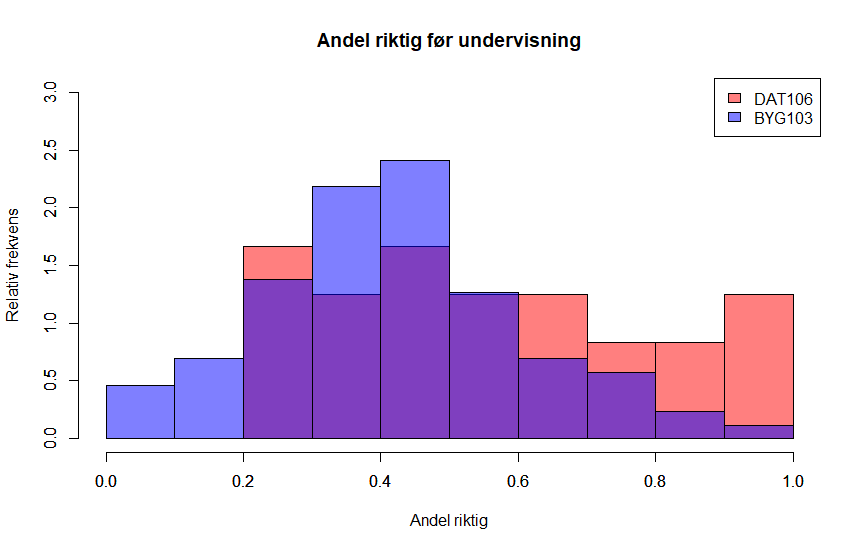
\includegraphics[width=.48\textwidth]{./preScoreAll}
	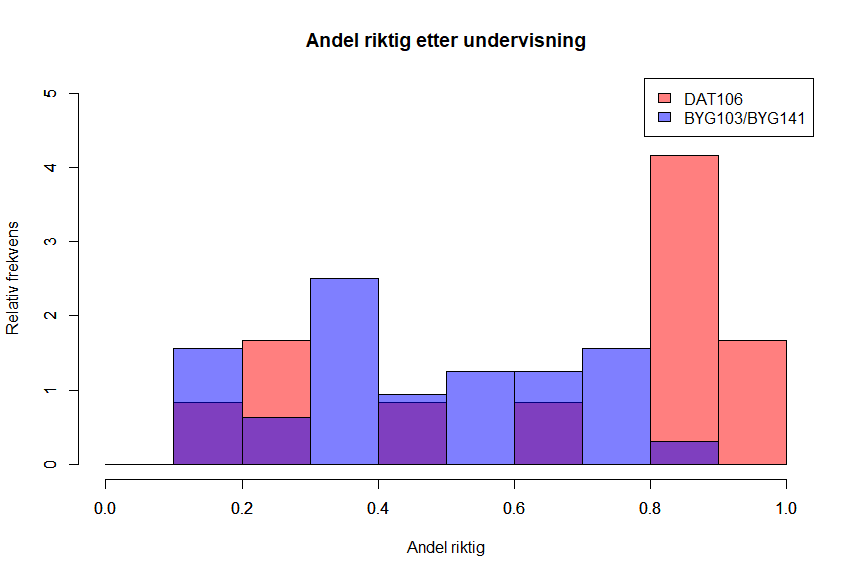
\includegraphics[width=.48\textwidth]{./postScore}
	\caption{Sammenligning av testresultater for studenter fra kursene DAT106 og  BYG103/BYG141 før (venstre) og etter (høyre) undervisningsperioden. Histogrammet med før-resultater 
baserer seg på flere studenter enn histogrammet for etter-resultater siden færre studenter valgte å delta på testen andre gang.}
	\label{fig:testScore}
\end{figure}

\begin{figure}[p]
	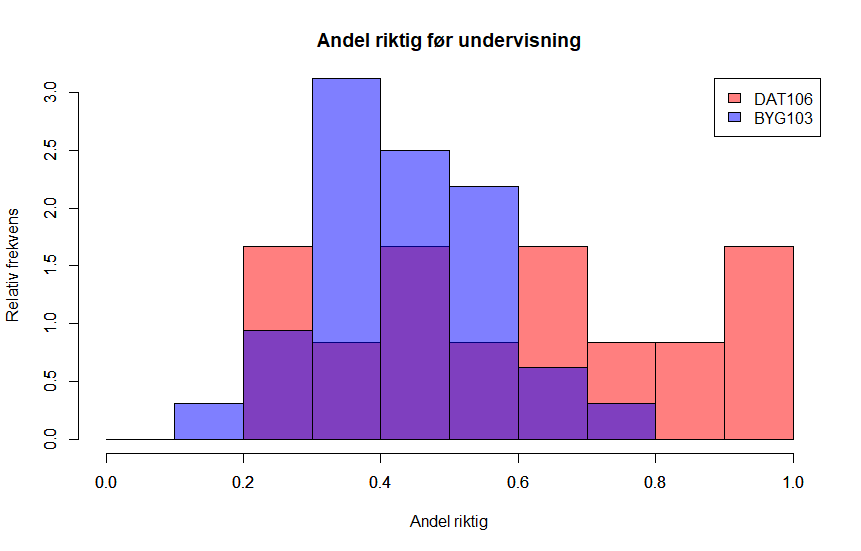
\includegraphics[width=.48\textwidth]{./preScore}
	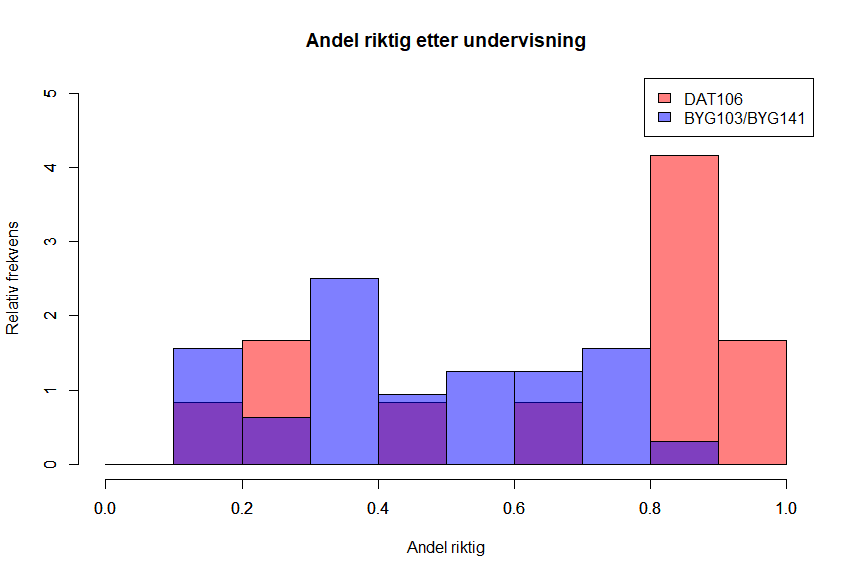
\includegraphics[width=.48\textwidth]{./postScore}
	\caption{Sammenligning av testresultater for studenter fra kursene DAT106 og  BYG103/BYG141 før (venstre) og etter (høyre) undervisningsperioden. Kun studenter som deltok på både før- og etter-testene er inkludert i histogrammene.}
	\label{fig:testScoreMatch}
\end{figure}

For de studentene som deltok på både før- og etter-testen er utviklingen i resultat vist i figur \ref{fig:forbedring}. Histogrammet til venstre viser absolutt forbedring, altså $S_\text{etter}-S_\text{før}$ der $\eta_\text{abs} = S_\text{før}$ og $S_\text{etter}$ er andel riktig i testen henholdsvis før og etter undervisningsperioden. Histogrammet til høyre viser den relative forbedringen definert som
\begin{displaymath}
	\eta_\text{rel} = \frac{S_\text{etter}-S_\text{før}}{1 - S_\text{før}}.
\end{displaymath}
Den relative forbedringen kan tolkes som hvor stor andel av spørsmålene som var feil besvart første gang som ble riktig besvart andre gang. Merk at denne variablen har en svakhet for studenter som hadde et svært godt resultat ved første test: Hvis en av disse studenten gjør kun \'en feil mer i andre forsøk enn i første forsøk får den relative forbedringen en stor negativ verdi.
\begin{figure}[p]
	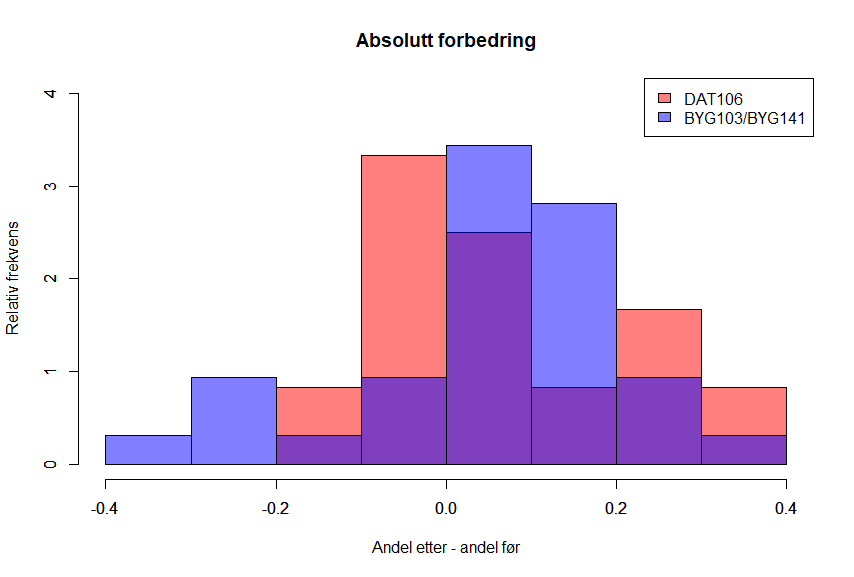
\includegraphics[width=.48\textwidth]{./absForbedring}
	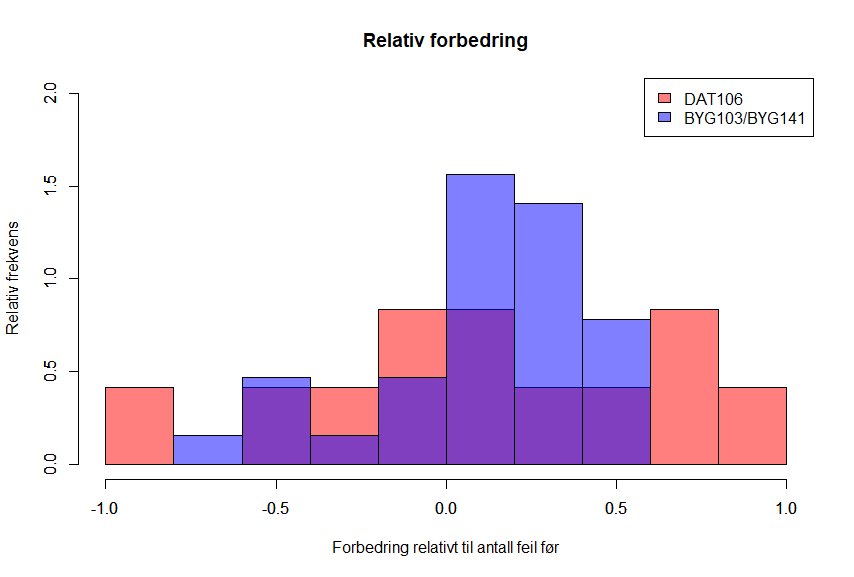
\includegraphics[width=.48\textwidth]{./relForbedring}
	\caption{Sammenligning av forbedring fra test før undervisningsperiode til test etter undervisningsperiode for DAT106 og BYG103/BYG141. Venstre histogram viser absolutt forbedring, mens høyre histogram viser den relative forbedringen (definert i teksten). }
	\label{fig:forbedring}
\end{figure}
For å kunne undersøke hvorvidt studentens forkunnskaper påvirker hvor godt resultat de ulike gir er det i figur \ref{fig:scatter} vist resultat av før-testen plottet mot absolutt forbedring (venstre) og relativ forbedring (høyre). 
\begin{figure}[p]
	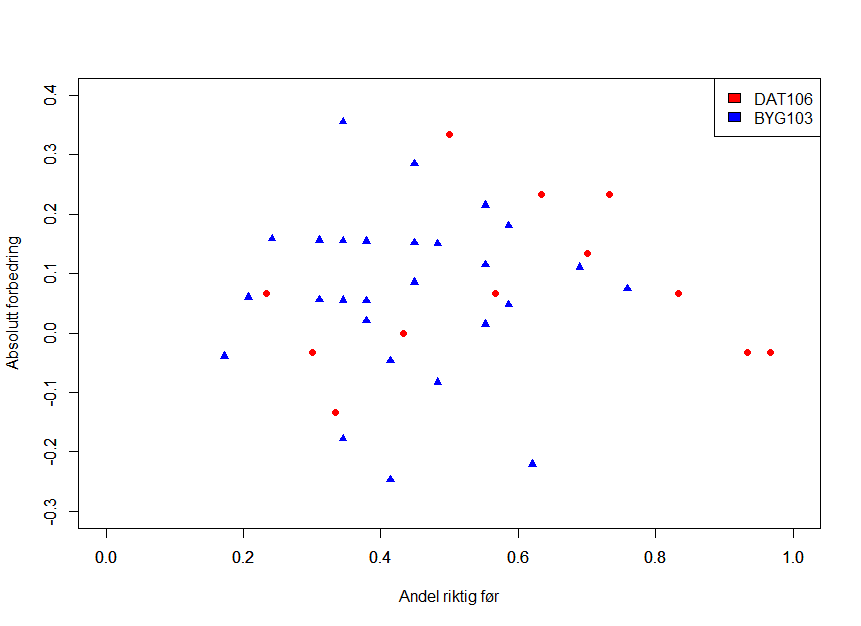
\includegraphics[width=.48\textwidth]{./absoluttForbedringScatter}
	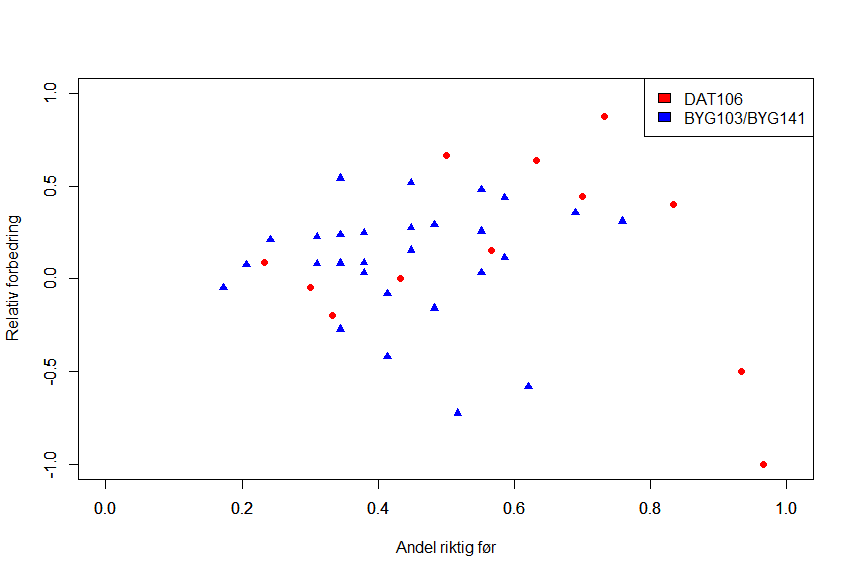
\includegraphics[width=.48\textwidth]{./relativForbedringScatter}
	\caption{Spredningsplott som viser sammenheng mellom andel riktig på test før undervisningsperioden og absolutt forbedring (venstre) eller relativ forberding (høyre).}
	\label{fig:scatter}
\end{figure}

\subsubsection{Betydningen av studiebakgrunn}
Datasettet som er samlet inn er ikke stort nok til å gjøre en studie av i hvilken grad ulike aspekter ved studentenes bakgrunn før de startet på DAT106 eller BYG103/BYG141 påvirker læringsutbyttet. Derfor begrenser dette avsnittet seg til å presentere resultater for sammenhengen mellom studentenes bakgrunn og resultatene de oppnådde på testen før undrevisningsperioden. Dette har imidlertid egen-interesse utover hovedmålsetningen med prosjektet mitt, og er derfor verdt å undersøke. Datasettet som er brukt for denne delen av studien er matchPreData. I noen tilfeller er imidlertid ikke alle studentene i dette datasettet inkludert, da matchingen ikke krever at de har svart på alle spørsmålene om studiebakgrunn.

Figur \ref{fig:fysmat} viser andel riktig på før-testen for studenter med/uten Fysikk 2 (venstre). Dette er kurs som ikke utgjør en del av opptakskravet for ingeniørstudiene, men som gir studentene en større fordypning i fysikk og matematikk enn minimumskravet. Det er dermed interessant å undersøke om dette påvirker testresultatene.
\begin{figure}[p]
\begin{center}
	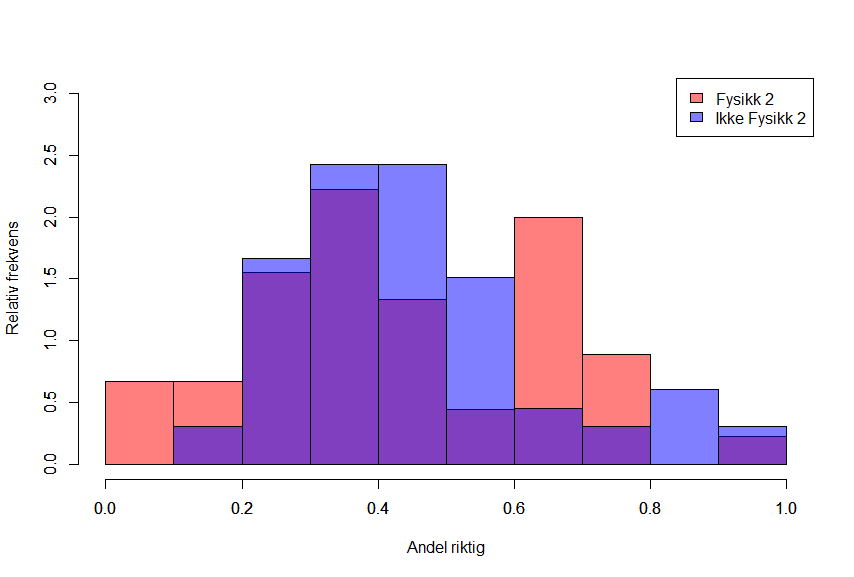
\includegraphics[width=.48\textwidth]{./fys2}
%	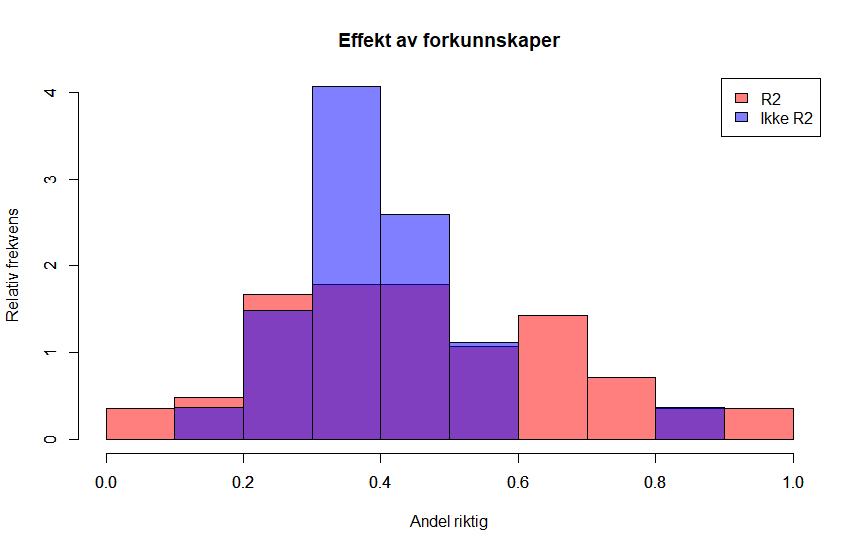
\includegraphics[width=.48\textwidth]{./r2}
\end{center}
	\caption{Sammenligning av resultater på testen før undervisningsperioden for studenter som har tatt kurset Fysikk 2 på videregående skole med de studenten som ikke har tatt dette kurset.}
	\label{fig:fysmat}
\end{figure}

Elever som ikke har tilstrekkelig fordypning i matematikk og fysikk fra videregående kan oppnå påkrevd kompetanse for å starte på ingeniørstudier gjennom å ta enten forkurs eller realfagskurs {\color{red}[Fyll inn detaljer. Snakk med Kristine]}. Figur \ref{fig:forkurs} viser andel riktig på før-testen for studenter som har bakrunn fra enten realfagskurs (venstre) eller forkurs (høyre). I begge tilfeller er resultatene sammenlignet med studenter som er tatt opp på studiet med tilstrekkelig fordypning i matematikk og fysikk fra videregående skole.
\begin{figure}[p]
	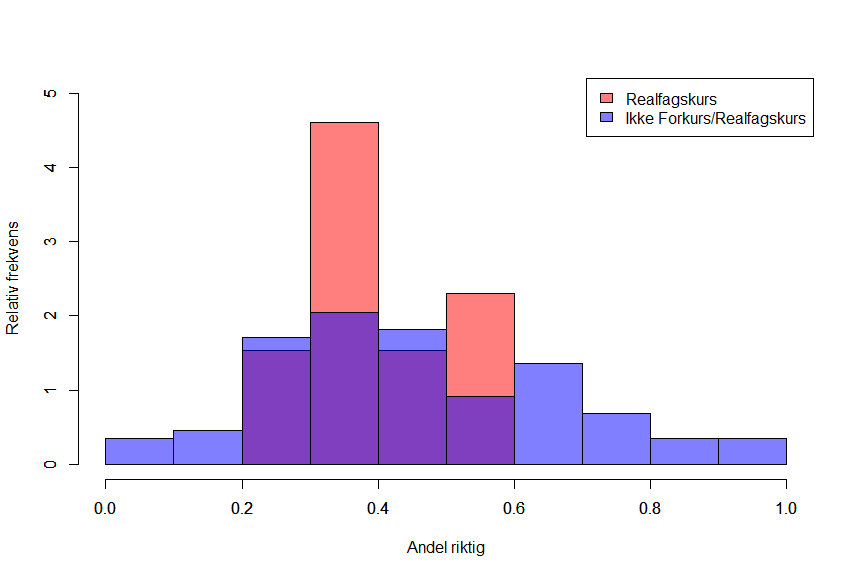
\includegraphics[width=.48\textwidth]{./real}
	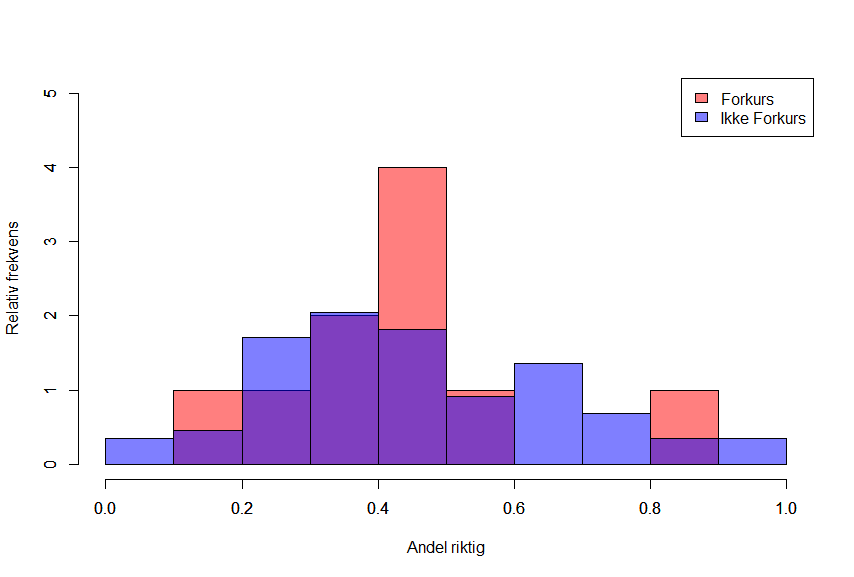
\includegraphics[width=.48\textwidth]{./forkurs}
	\caption{ Sammenligning av resultater for studenter som har tilstrekkelig matematikk- og fysikk-bakgrunn fra videregående skole (blå) med studenter som har tatt realfagskurs (venstre) eller forkurs (høyre) for å oppfylle opptakskravet til ingeniørstudier (rød).}
	\label{fig:forkurs}
\end{figure}

Matematikk er et viktig verktøy i fysikk-faget, og det er derfor interessant å undersøke om det er korrelasjon mellom hvor godt studenter mestrer matematikk og hvordan de presterer på fysikk-testen. Som proxy på matematikk-nivået til studentene har jeg brukt karakteren de fikk i matematikk-kurset MAT100/MAT108/MA2-100\footnote{Det er ulike matematikk-kurs for de ulike studieprogrammene og studiestedene, men alle disse tre kursene er tilstrekkelig like til at sammenligningen blir representativ}. Gjennomsnittlig andel riktig på testen i denne studien fordelt på karakterene A-F er vist i figur \ref{fig:mat100}. På histogrammet er det også vist en estimator for usikkerheten til gjennomsnittet av de ulike populasjonene. Merk at det kun er fire studenter som hadde karakteren F. En av studentene med karakteren F gjorde det svært bra på testen og trekker derfor gjennomsnittet langt oppover. Det er også verdt å notere at estimatoren for usikkerhet selv er svært usikker når populasjonen er så liten som i dette tilfellet.
\begin{figure}[p]
\begin{center}
	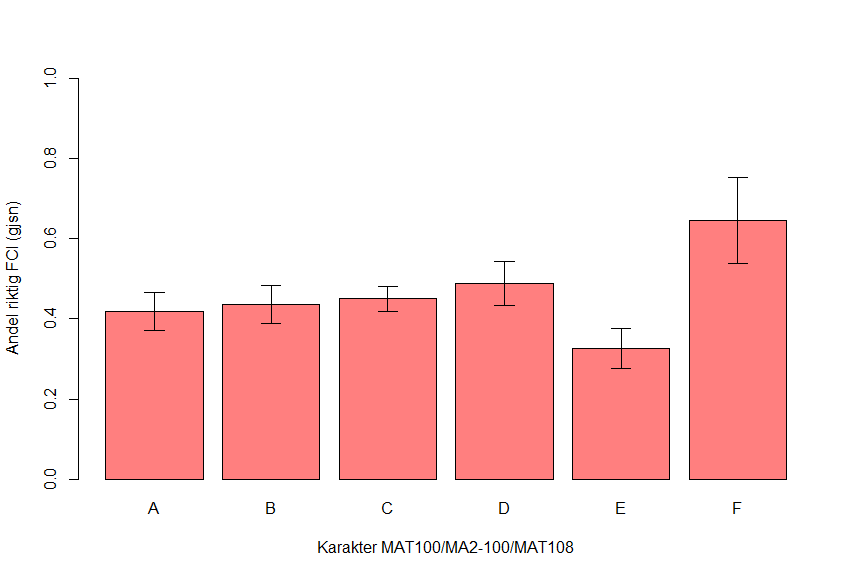
\includegraphics[width=.48\textwidth]{./mat100}
\end{center}
	\caption{Gjennomsnittlig andel riktig fordelt per karakter i matematikk-kursene MAT100/MAT108/MA2-100. Merk at for karakteren F er gjennomsnittet trukket langt oppover på grunn av at kun fire studenter hadde denne karakteren, og \'en av dem gjorde det svært bra på testen.}
	\label{fig:mat100}
\end{figure}



\section{Diskusjon av resultatene}

\subsection{Sammenligning av tradisjonell forelesning og omvendt klasserom}
Det primære målet for denne studien var å undersøke om ''omvent klasserom''---som en representant for studentaktive læringsformer---gir bedre læringsutbytte for studentene enn ''tradisjonell forelesning''. En sammenligning av resultatene fra testen før undervisningsperioden og etter undervisningsperioden, vist i figurene \ref{fig:testScore}-\ref{fig:testScoreMatch}, viser at begge studentgruppene har bedret resultatet sitt---hvilket selvfølgelig er målet med undervisningen uansett hvordan den er organisert. Det tydeligste bildet får vi fra figur \ref{fig:testScoreMatch} der det er nøyaktig den samme studentpopulasjonen som er brukt i histogrammet for resultater før og etter testen. Ved å sammeligne på denne måten tar vi vekk utvalgsbiasen som kan komme dersom det er en korrelasjon mellom resultatet på første test og hvorvidt en student velger å delta på andre test eller ikke. Sammenligning av første histogram i henholdsvis figur \ref{fig:testScore} og \ref{fig:testScoreMatch} viser at det til en viss grad er en slik utvalgsbias til stede: Spesielt i BYG103/BYG141 ser vi at en større andel av studentene med de sterkeste og de svakeste resultatene på første test valgte å ikke ta andre test. I DAT106 er utvalgsbiasen mindre, men også her ser vi en tendens til at studenter fra svakeste halvpart på første test i større grad valgte å ikke ta andre test. 

For å evaluere endringen mellom første og andre test er det nyttig å studere histogram som viser forbedringen som vist i figur \ref{fig:forbedring}. Ut fra histogrammene kan vi se at gruppen med omvent klasserom (DAT106) har i gjennomsnitt noe bedre fremgang enn gruppen med forelesninger (BYG103/141), men forskjellen er ikke stor. Størrelsen på forskjellen kan vi kvantisere ved å se på gjennomsnittlig forbedring ($\hat{\mu}$) samt en estimator for standardavviket ($\hat{\sigma}_\mu = \sigma/\sqrt{n}$) til fordelingen for de to gruppene. Disse beregnes til å være
\begin{displaymath}
\begin{aligned}
	\hat{\mu}_\text{DAT106} &= 0.075,\quad\quad \hat{\sigma}_{\mu,\text{DAT106}} &= 0.039, \\
	\hat{\mu}_\text{BYG103} &= 0.048,\quad\quad \hat{\sigma}_{\mu,\text{BYG103}} &= 0.028. \\
\end{aligned}
\end{displaymath}
Vi ser at spredningen i forbedringen til de ulike studentene innad i hver gruppe er for stor til at tallmaterialet som er tilgjengelig kan brukes til å konkludere med at den ene undervisningsformen har gitt bedre resultater enn den andre. Om vi fortsetter å bruke antakelsen at usikkerheten på estimatoren til standardavviket skalerer som $1/\sqrt{n}$ der $n$ er antall studenter i gruppen viser disse tallen at det hadde vært behov for omlag tre ganger så mange studenter i studien for å kunne få et signifikant resultat.

Selv om tallmaterialet fra studien ikke gir grunnlagt for å svare på det primære spørsmålet jeg ønsket å undersøke er det verdt å studere det innsamlete datasettet videre for å se om det er andre interessante konklusjoner det er mulig å trekke. Figur \ref{fig:scatter} fremstiller sammenghengen mellom resultat på testen før undervisning og forbedringen til testen etter undervisning. Dette gir mulighet til å undersøke om undervisningen har ulik effekt på studenter med ulikt utgangspunkt. På samme måte som i figur \ref{fig:forbedring} viser også denne figuren absolutt forbedring i venstre diagram og relativ forbedring i høyre diagram. Diagrammet med relativ forbedring er det som er enklest å tolke. For gruppen med forelesninger (BYG103/BYG141) ser vi at det ikke er noen sammenheng mellom utgangspunktet og hvor mye studentene forbedret seg. Det ser altså ut til at effekten av forelesningene er like stor for både de sterkeste og svakeste av studentene. Her er det imidlertid verdt å minne på at tallmaterialet er svært begrenset, så denne konklusjonen er meget svak.

Resultatet fra gruppen med omvendt klasserom (DAT106) er litt mer komplisert---først og fremst på grunn av de to studenten med stor negativ relativ forbedring. Som diskutert ovenfor er dette en artefakt som kan oppstå med denne måten å kvantisere forbedringen mellom første og andre test. Siden den relative forbedringen er definert som 
\begin{displaymath}
	\eta_\text{rel} = \frac{S_\text{etter}-S_\text{før}}{1 - S_\text{før}}.
\end{displaymath}
der $S_\text{før/etter}$ er andel riktig i testen før/etter undervisning, vil selv en liten negativ endring i teller gi et stort utslag dersom $S_\text{før}$ er nær 1 slik at nevner er liten. Dette gjør at det er rimelig å tillegge disse datapunktene liten vekt. Hvis vi fullstendig ignorerer de to datapunktene med stor negativ relativ forbedring ser vi at det er en tydelig positiv korrelasjon mellom andel riktig i testen før undervisningsperioden og den relative forbedringen. Denne positive korrelasjonen betyr at det er studentene med best utgangspunkt som forbedret seg mest i løpet av undervisningsperioden. Igjen er konklusjonen svak på grunn av det lille datasettet, men studien tyder på at omvendt klasserom fungerer best for studentene som kom til kurset med det beste utgangspunktet. 

\subsection{Sammenheng mellom test-resultater og studiebakgrunn}
I denne delen studerer jeg sammenhengen mellom resultater på testen før undervisningsperioden og ulike aspekter ved studentenes bakgrunn før kurset DAT106/BYG103/BYG141. For å redusere effekten av statistiske fluktuasjoner mest mulig behandler jeg her alle studentene som \'en gruppe i stedet for å dele dem inn etter hvilket kurs de tar. Siden denne delen av analysen kun ser på resultatene fra testen før undervisningsperioden, og siden det kun er en liten forskjell i hvor godt studentene i de to gruppene gjorde det på den første testen introduserer ikke dette noen problematisk bias.

\subsubsection{Fysikk 2}
I rammeplanen for ingeniørutdanning \cite{rammeplan} står det:
\begin{quote}I ingeniørutdanning er det viktig å forstå fysisk lover. Både klassisk og moderne fysikk inngår i faget Fysikk 1 i videregående opplæring. Fysikk i ingeniørutdanning skal bygge videre på dette. Fysikkundervisningen for alle studieretninger må inneholde en konsolidering og fordypning av studentenes kunnskaper i klassisk ([\ldots]) og moderne fysikk.\end{quote}
Fysikk 1 er det første fordypningsfaget i fysikk (2.~klasse i videregående skole) og er spesielt nevnt siden dette faget utgjør en del av opptakskravene til ingeniørstudier. I tillegg tilbys også faget Fysikk 2 (3.~klasse videregående skole) som delvis bygger videre på Fysikk 1, men også introduserer en del nye emner. Det kreves ikke Fysikk 2 ved opptak til ingeniørstudier. 

Testen som er brukt i denne studien omhandler kun emner som er en del av Fysikk 1, men dette er emner som konsolideres og videreutvikles i Fysikk 2. Det er derfor grunn for å forvente at studenter som har vært gjennom Fysikk 2 vil få bedre resultater på testen før undervisning enn de studentene som kun har Fysikk 1, eventuelt realfagskurs/forkurs (som har tilsvarende pensum som Fysikk 1). Som vi kan se fra figur \ref{fig:fys2} er dette imidlertid ikke tilfellet. Om vi på samme måte som ovenfor beregner gjennomsnittlig andel riktig på test før undervisningsperioden og estimert usikkerhet på dette finner vi
\begin{displaymath}
\begin{aligned}
	\hat{\mu}_\text{med Fysikk 2} &= 0.44\pm 0.03, \\
	\hat{\mu}_\text{uten Fysikk 2} &= 0.45\pm 0.02,
\end{aligned}
\end{displaymath}
som bekrefter vurderingen ut fra histogrammet, nemlig at vi ikke kan måle noen forskjell i resultater for studenter med og uten Fysikk 2. 


\subsubsection{Realfagskurs/forkurs}
Studenter som ikke oppfyller kravet om matematikk-kursene R1 og R2 og fysikk-kurset Fysikk 1 fra videregående skole må ta enten realfagskurs eller forkurs for å være kvalifisert til opptak på et ingeniørstudium. Siden dette er studenter som har valgt bort å ikke ta disse kursene på videregående skole er det rimelig å anta at de i gjennomsnitt er mindre interessert i matematikk og fysikk enn de øvrige studentene. På den annen side er undervisningen i forkurset/realfagskurset langt mer komprimert enn på videregående skole, slik at studenter som har gjennomført dette har vært nødt til å jobbe mye over en kort tid med matematikk og fysikk. Disse betraktningen som virker i motsatt retning på hvilken forventning man vil ha til denne studentgruppen gjør det spesielt interessant å studere hvordan de presterer på testen i denne studien.

Figur \ref{fig:forkurs} viser at spredningen i test-resultater er langt mindre blant både studentene med forkurs og med realfagskurs enn den øvrige studentpopulasjonen. Antallet studenter med forkurs (10) og realfagskurs (13) er for lite til å kunne avgjøre om denne forskjellen skyldes studiebakgrunnen eller om det er bare er en statistisk effekt som skyldes den lille populasjonen. Når vi ser på gjennomsnittlig andel riktige i de tre gruppene (realfagskurs, forkurs, andre---det vil si studenter med R1+R2 og Fysikk 2) er det kun små forskjeller:
\begin{displaymath}
\begin{aligned}
	\hat{\mu}_\text{Realfagskurs} &= 0.39\pm 0.03 \\
	\hat{\mu}_\text{Forkurs} &= 0.43\pm0.06 \\
	\hat{\mu}_\text{Andre} &= 0.46\pm 0.02
\end{aligned}
\end{displaymath}
Forskjellen mellom gruppen med realfagskurs og andre er stor nok til at vi kan konkludere med at det er en signifikant forskjell. Sammenligning av andre kombinasjoner av de tre gruppene viser ingen signifikante forskjeller.

\subsubsection{Matematikk-kurs fra tidligere i studiet}
I første semester av studiet tar studentene et matematikk-kurs som blant annet inkluderer temaer (derivasjon, integrasjon, vektorregning) som er viktig for å gjøre beregninger i fysikk-faget. Kurset har ulik fagkode og noen mindre forskjeller i pensum for de ulike studieretningene og studiestedene (DAT106: MAT108, BYG103: MAT100, BYG141: MA2-100), men den delen av pensum som er av størst betydning for fysikk-faget er inkludert i alle varianter. Studentene i DAT106 har i tillegg hatt et annet matematikk-kurs (MAT101) tidligere i studiet, men pensum i dette kurset er i svært liten grad relevant for den delen av fysikk-faget som denne studien omhandler. Spørsmålene i testen som er brukt i denne studien krever ingen beregninger, kun fysisk forståelse. Det er derfor ingen direkte kobling mellom det de har lært i matematikk-kurset og spørsmålene de blir bedt om å svare på i denne studien. Det er likevel fristende å anta at studenter som er gode i matematikk også er gode i fysikk, siden fysikk generelt er et fag som har svært sterk kobling til matematikken. Resultatene som er vist i figur \ref{fig:mat100} viser imidlertid ingen korrelasjon mellom matematikk-karakter og testresultat. Publiserte resultater fra lignende studier har funnet en korrelasjon mellom studenters matematikk-nivå og evnen til å lære fysikk på et konseptuelt nivå~\cite{5c27a2a258c342bc822a508f17d2b0da}, men det er også funn som viser at matematikk-nivået alene ikke er en god prediktor for resultatet i et fysikk-kurs~\cite{VINITSKYPINSKY2014611}. Dette er et tema som ville vært interessant å følge opp, blant annet for å undersøke om hvordan matematikk-pensum og -undervisningen er organisert påvirker i hvilken grad studentene klarer  å nyttegjøre seg av matematikken i andre fag som for eksempel fysikk.

\section{Diskusjon av studiedesign}
\label{sec:studiedesign}
Siden studien endte opp med et tallmateriale som ikke var tilstrekkelig til å gi et signifikant resultat angående det primære spørsmålet er det verdt å foreta en vurdering av studiedesignet og komme med noen forslagt til hvordan det kan forbedres til en eventuelt senere studie. Hovedproblemet med studien er at antallet studenter som deltok var for lavt. Det lave deltakertallet skyldes flere faktorer:
\begin{itemize}
\item
Av praktiske årsaker har jeg kun involvert de studentene jeg selv foreleste for i inneværende semester i studien. Dette gjør at det er et svært begrenset antall studenter som var potensielle deltakere. Spesielt i kurset DAT106 er dette en begrensende faktor siden det er langt færre studenter per årskull på dataingeniørlinjen enn på bygg- og anleggsingeniørlinjen.
\item
Testene ble utført i forbindelse med forelesninger. Dette kan virke begge veier---det gjør det enkelt for de som møter til forelesning å velge å være med på testen, men samtidig er det en relativt stor andel av studentene som ikke går på forelesning og av den grunn ikke deltok.
\item
Det var frivillig å delta på testene og studentene hadde ingen egeninteresse av å delta utover at de fikk en anledning til å øve seg på å løse fysikk-oppgaver.  Spesielt på testen etter undervisningsperioden ser denne faktoren ut til å vært av stor betydning, da langt færre studenter var med på denne testen sammenlinget med testen før undervisningsperioden.
\item
Behovet for å koble svarene fra samme student på de to testene samtidig som testen skulle være anonym var en utfording. Løsningen som ble valgt var at studentene logget inn med et selvvalgt ''nick-name'' som de måtte bruke ved begge testene. Selv om listen over ''nick-names'' som var brukt ved første test ble gjort tilgjengelig ved andre test var det en god del mangel på overlapp. Dermed var det en del av det innsamlede datamaterialet som ikke kunne brukes til analysen for å besvare det primære spørsmålet i studien.
\end{itemize}
Det viktigste bidraget til å øke data-mengden er å øke antall potensielle deltakere i studien. I praksis vil det si at studien måtte utføres over flere år slik at flere kull blir testet. I diskusjonen av resultatene ble det vist at for å kunne forvente å få signifikante resultater trengs det minst en tredobling av antall studie-deltakere. Dette betyr at studien antakelig må gå over tre år---noe som er relativt omfattende, men ikke helt urealistisk. Hvis andelen av studentene fra hvert årskull som deltar kan økes vesentlig er det mulig at det er tilstrekkelig å gjøre studien over to år. Fordi testen skal gjøres uten diskusjon eller bruk av hjelpemidler, og fordi testspørsmålene skal gjøres utilgjengelig igjen straks etter at testen er gjennomført er det mer eller mindre nødvendig at testen gjennomføres med studentene samlet i ett rom. Det er derfor neppe aktuelt å gjennomføre testen på annet vis enn i forbindelse med forelesning. Det er også vanskelig å gjøre testen obligatorisk for studentene da dette vil kreve at den kommer inn som en del av de obligatoriske kravene i emnebeskrivelsen til kurset. Dermed er det de to siste punktene på listen ovenfor som er mest aktuelle å ta tak i. Egeninteressen til studentene for å delta i studien er til stede, men det kreves nok en del overbevisning for at de skal innse det tidlig i semesteret mens det fremdeles er lenge igjen til eksamen. 

Det siste punktet på listen er et teknisk problem som relativt enkelt kan løses selv om det krever en ikke ubetydelig engangs-innsats. Det kan programmeres en egen innlogging der studentene logger inn med for eksempel studentnummer som blir behandlet av en hash-algoritme før det lagres. Siden en hash-algoritme er enveis vil dette gi en unik identifikator for hver student som er lik ved begge tester, men som ikke kan spores tilbake til studentnummeret. Dermed er anonymiteten ivaretatt samtidig som sannsynligheten for manglende kobling mellom resultatet fra første og andre test er tilnærmet eliminert.

Et  aspekt ved studiedesignet som har stor betydning for i hvilken grad resultatene kan generaliseres er hvordan ''tradisjonell forelesning'' og ''omvendt klasserom'' defineres. Dette kan ha stor betydning for utfallet av studien, og hvis studien skal utføres over flere år, eventuelt med flere undervisere involvert, er det av stor betydning at undervisningsformene er tilstrekkelig klart definert. 

I denne studien har ''tradisjonell forelesning'' inkludert noen interaktive elementer i form av quizer besvart per mobiltelefon eller datamaskin, og regne-eksempler der studentene har blitt bedt om å forsøke selv før eksempelet blir gjennomgått. Selv om disse interaktive elementene utgjøre en liten andel av undervisningstiden har de en viktig funksjon ved at monotonien blir brutt, og at studentene får et mer aktivt forhold til lærestoffet. Det kan tenkes at forelesning med og uten interaktive elementer vil gi ulikt læringsutbytte, men uten å ha undersøkt dette vil det bare bli en spekulasjon.

\section{Konklusjon}
Jeg har her presentert en studie som undersøker om det er forskjell i læringsutbytte mellom tradisjonelle forelesninger og studentaktiv undervisning, her representert ved en variant av omvendt klasserom. Resultatene fra studien viser ingen signifikant forskjell mellom læringsutbyttet fra de to undervisningsformene. Det vises at for å kunne forvente et signifikant resultat må antallet studenter som deltar i studien minst tredobles. Svakheter i gjennomføring av datainnsamlingen, noe som var medvirkende til det lave deltakertallet, ble diskutert i avsnitt \ref{sec:studiedesign}. 

Med utgangspunkt i datasettet som ble samlet inn for å svare på det primære spørsmålet i studien har jeg også studert studentenes ferdighetsnivå i fysikk ved begynnelsen av kurset målt opp mot ulike aspekter ved deres studiebakgrunn. Den eneste signifikante effekten som ble funnet er at studenter som er tatt opp på ingeniørstudiet med realfagskurs i stedet for R1+R2 og Fysikk 1 fra videregående skole er i gjennomsnitt på et lavere nivå enn studenter med tilstrekkelig matematikk- og fysikk-bakgrunn fra videregående skole. Det ser også ut til å være en mindre spredning i ferdighetsnivået til studentene som er tatt opp på grunnlag av forkurs eller realfagskurs enn de studentene som har tilstrekkelig matematikk- og fysikk-bakgrunn fra videregående skole.

\appendix
\section{Merknader til gjennomføring av testene}
Her dokumenteres enkelte feil som ble gjort i forbindelse med datainnsamlingen. 
\subsection{BYG103/BYG141}
\begin{itemize}
\item
Ved begge testene satt studentene for tett til å hindre kommunikasjon eller at de så på hverandres svar. Jeg oppfordret på forhånd til å jobbe selvstendig uten diskusjon. Dette ble langt på vei, men ikke fullstendig etterlevd.
\item
En av oppgavene manglet figuren som var avgjørende for å forstå spørsmålet da testen ble gjennomført første gang. En håndtegnet versjon av figuren ble gjort tilgjengelig få minutter etter at dette ble oppdaget.
\item
Nummerering av oppgavene var feil da testen ble gjennomført første gang. Dette laget forvirring i et tilfelle der det ble vist tilbake til en figur som hørte til en tidligere oppgave. Jeg ga muntlig beskjed til alle straks feilen ble oppdaget, men det kan likevel ha forårsaket noe forvirring eller tidstap.
\item
En av oppgavene manglet det riktige svaralternativet (kun fire av de fem alternativene som skulle vært tilgjengelig var inkludert) da testen ble gjennomført første gang. I analysen er dette spørsmålet tatt bort når andel riktig regnes ut for før-testen til BYG103/BYG141. I ettertesten og begge testene til DAT106 er spørsmålet inkludert i beregningen. Dette vil introdusere en liten bias dersom dette spørsmålet oppfattes som enklere eller vanskeligere enn gjennomsnitt av spørsmålene.
\end{itemize}

\subsection{DAT106}
\begin{itemize}
\item
Ved begge testene satt studentene for tett til å hindre kommunikasjon eller at de så på hverandres svar. Jeg oppfordret på forhånd til å jobbe selvstendig uten diskusjon. Dette ble langt på vei, men ikke fullstendig etterlevd.
\end{itemize}

\bibliographystyle{apalike}
\bibliography{referanser}
\end{document}